\documentclass[17pt]{memoir}
\usepackage{amsmath,amssymb}
\usepackage{import}
\usepackage{xifthen}
\usepackage{pdfpages}
\usepackage{transparent}
\usepackage{multicol}
% \usepackage{graphicx}
\pagestyle{empty}

\newcommand{\incfig}[1]{%
    \def\svgwidth{\columnwidth}
    \import{./}{#1.pdf_tex}
}


\begin{document}

% \includegraphics{drawing.pdf}

\begin{figure}[ht]
    \centering
    \incfig{drawing}
    \caption{Trigonometric functions}
    \label{fig:trig-functions}
\end{figure}

\begin{figure}[ht]
    \centering
    \incfig{trig_diagram}
    \caption{Trigonometric functions}
    \label{fig:trig-functions}
\end{figure}




\[ OA = 1 \]

\begin{multicols}{2}

\[ AC = \sin{\theta} \]
\[ OC = \cos{\theta} \]
\[ AB = \tan{\theta} \]

\columnbreak

\[ OB = \sec{\theta} \]
\[ OD = \csc{\theta} \]
\[ AD = \cot{\theta} \]

\end{multicols}

\newpage
\large

\begin{center}
Trigonometric Identities
\end{center}

\begin{multicols}{2}

{
\[ \sec{\theta} = \frac{1}{\cos{\theta}} \]
\[ \csc{\theta} = \frac{1}{\sin{\theta}} \]
\[ \cot{\theta} = \frac{\cos{\theta}}{\sin{\theta}} \]
}
{
\[ \sin^{2}\theta + \cos^{2}\theta = 1\]
\[ 1 + \cot^2 \theta = \csc^2 \theta \]
\[ 1 + \tan^2 \theta = \sec^2 \theta \]
}

\end{multicols}

\[ \sin(\alpha \pm \beta) = \sin\alpha \cos\beta \pm \sin\beta \cos\alpha \]
\[ \cos(\alpha \pm \beta) = \cos\alpha \cos\beta \mp \sin\alpha \sin\beta \]
\[ \tan(\alpha \pm \beta) = \frac{\tan \alpha \pm \tan \beta}{1 \mp \tan \alpha \tan \beta} \]

\end{document}
